\documentclass[a4paper,landscape]{article}
\usepackage[a4paper,landscape,margin=0.55cm]{geometry}
\usepackage{fontspec}
\usepackage{amsmath}
\usepackage{unicode-math}
\setmainfont{texgyreheros}[Extension=.otf,UprightFont=*-regular,BoldFont=*-bold,ItalicFont=*-italic,BoldItalicFont=*-bolditalic]
\setmathfont{texgyrepagella-math.otf}
\usepackage[table]{xcolor}
\usepackage{tikz}
\usetikzlibrary{arrows.meta,positioning,calc}
\usepackage{adjustbox}
\usepackage{array}
\pagestyle{empty}

\definecolor{ink}{HTML}{14213D}
\definecolor{trust}{HTML}{2F7A4F}
\definecolor{curious}{HTML}{C8611E}
\definecolor{untrusted}{HTML}{A23B3B}
\definecolor{chan}{HTML}{2F5F98}
\definecolor{soft}{HTML}{F3EFE6}
\definecolor{softblue}{HTML}{E6EEF8}
\definecolor{softgreen}{HTML}{E4F1E8}
\definecolor{softred}{HTML}{F6E3E1}
\definecolor{grey}{HTML}{6B7280}
\definecolor{bankc}{HTML}{1F6F8B}
\definecolor{keyc}{HTML}{8E2C6E}

\newcommand{\bk}{\tikz[baseline=(c.base)]\node[fill=bankc,text=white,rounded corners=1pt,inner sep=1.2pt,font=\bfseries\fontsize{5.6}{6}\selectfont] (c) {bank};}
\newcommand{\ek}{\tikz[baseline=(c.base)]\node[fill=keyc,text=white,rounded corners=1pt,inner sep=1.2pt,font=\bfseries\fontsize{5.6}{6}\selectfont] (c) {enclave key};}
\newcommand{\hd}[1]{{\bfseries #1}}
\newcommand{\sm}{\fontsize{7.4}{9.0}\selectfont}
\newcommand{\xs}{\fontsize{6.6}{8.1}\selectfont}

\tikzset{
  store/.style={draw=grey,fill=white,rounded corners=2pt,align=left,anchor=north west,inner sep=3pt},
  arr/.style={-{Stealth[length=4.5pt]},line width=0.9pt,ink},
  sarr/.style={-{Stealth[length=4.5pt]},line width=0.9pt,chan},
  albl/.style={font=\xs,fill=white,inner sep=1pt,align=center},
}

\begin{document}
\noindent
\begin{adjustbox}{max width=\linewidth,max totalheight=\textheight,center}
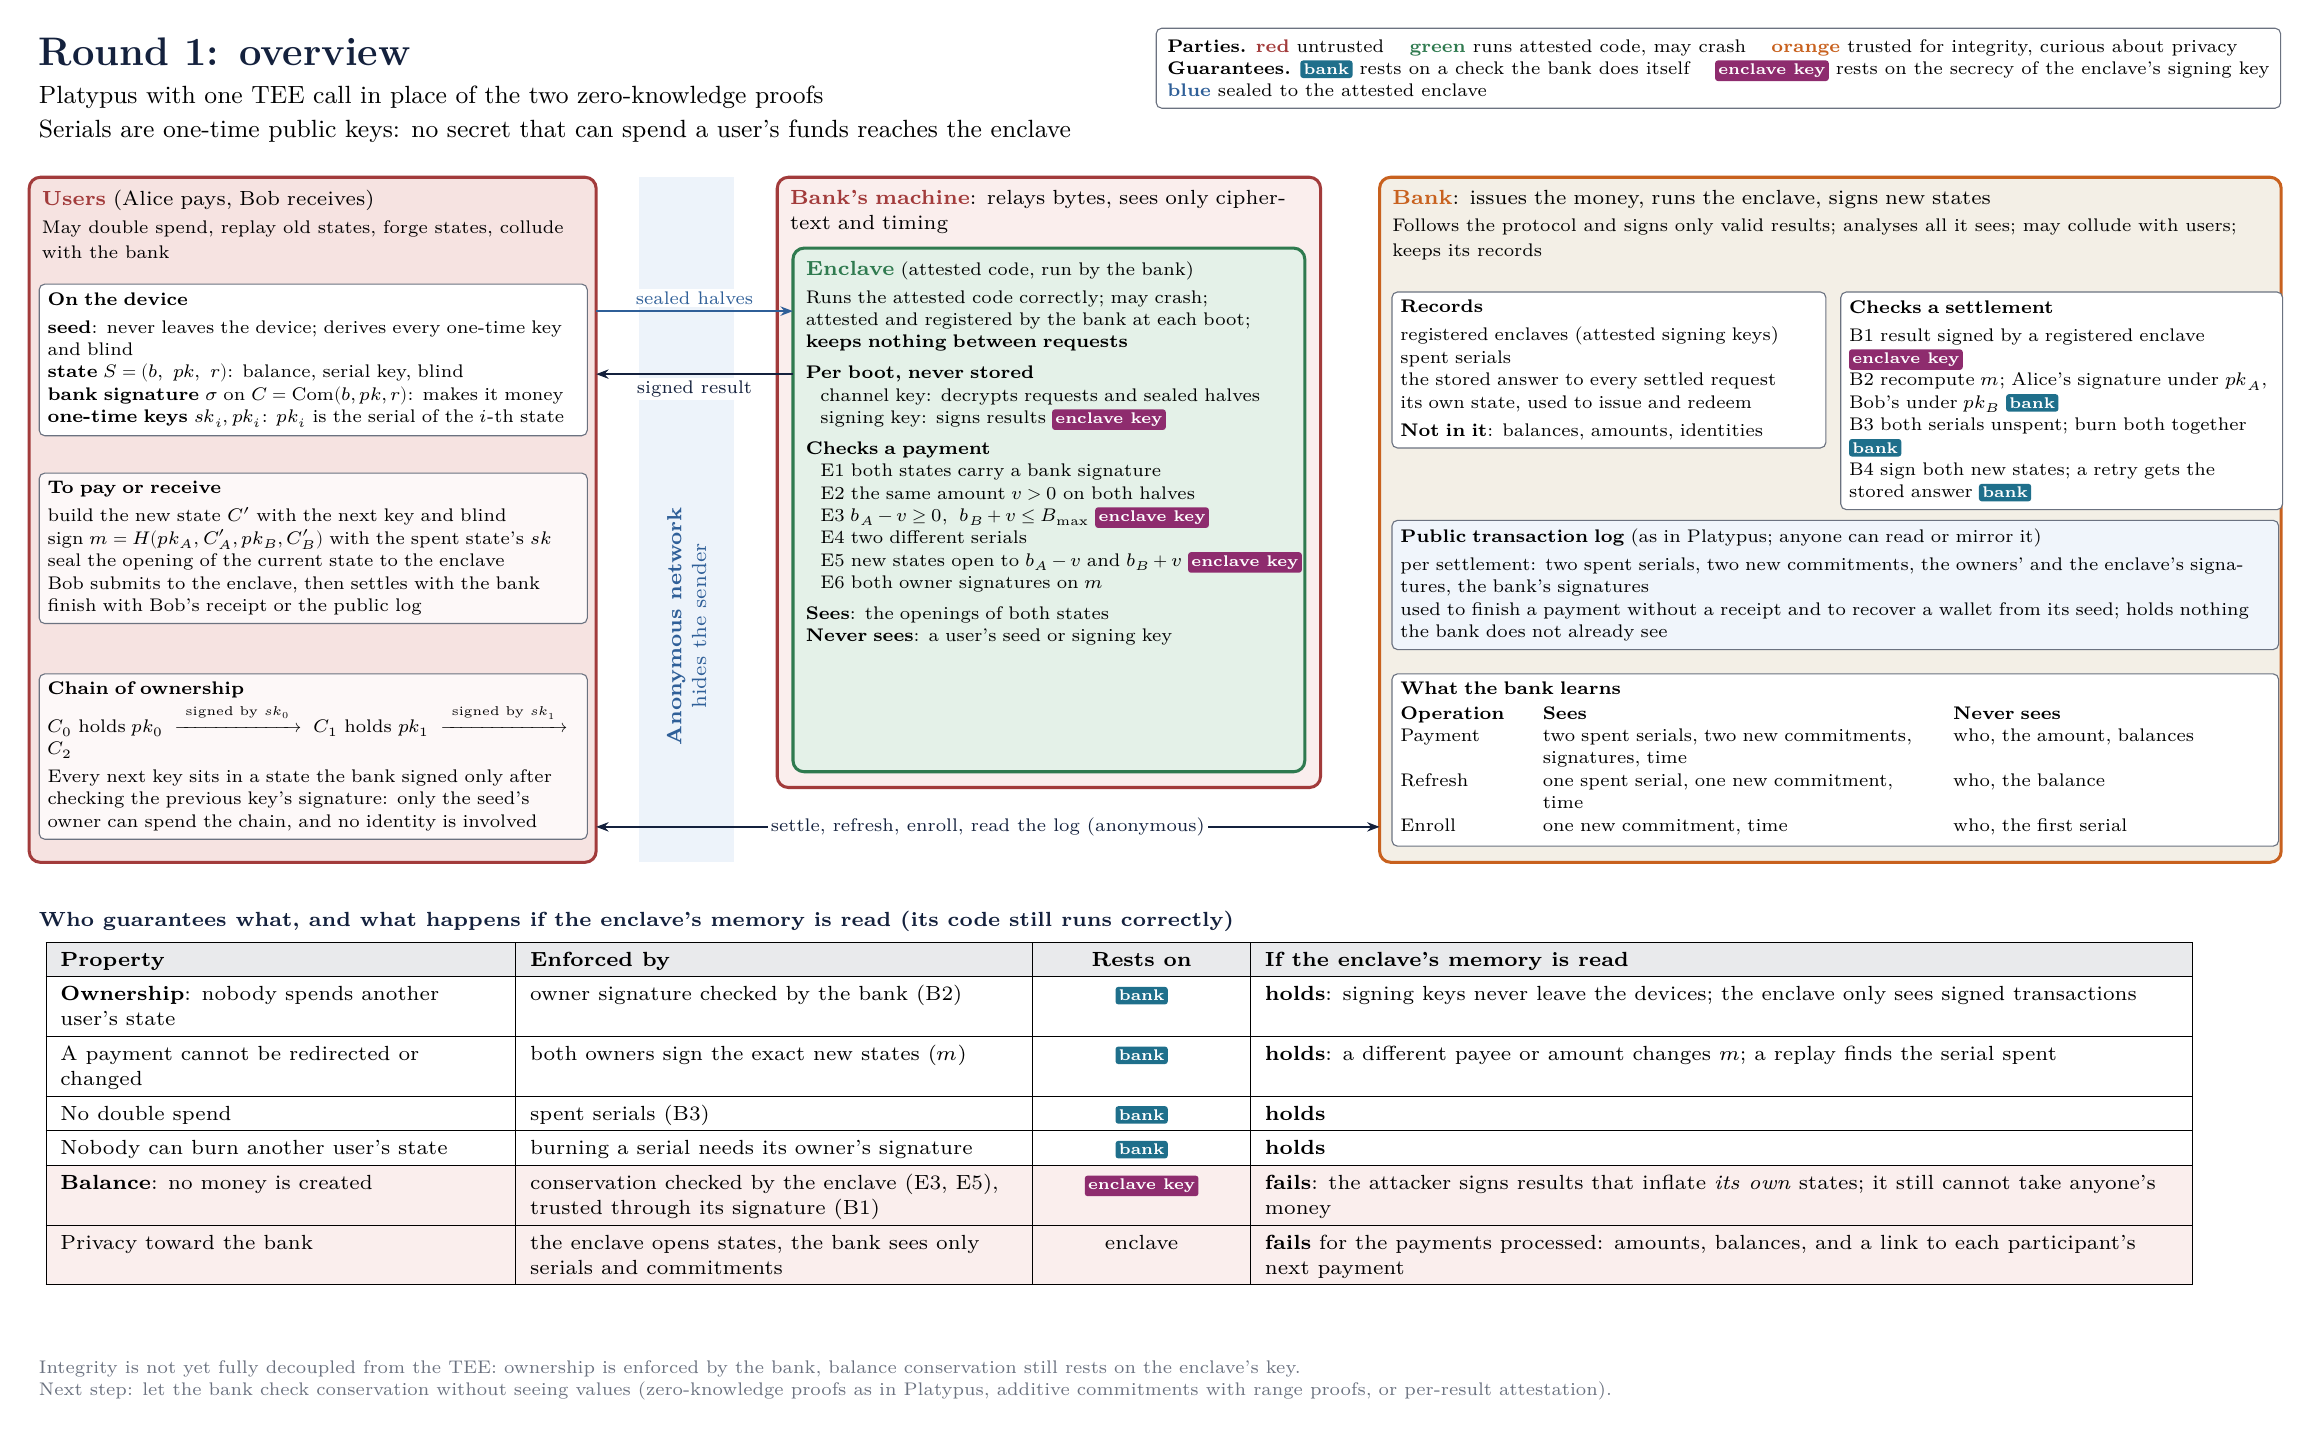
\begin{tikzpicture}[x=1cm,y=1cm]

\node[anchor=north west,align=left] at (0,20.2) {{\bfseries\Large\color{ink} Round 1: overview}\\[2pt]{\small Platypus with one TEE call in place of the two zero-knowledge proofs}\\{\small Serials are one-time public keys: no secret that can spend a user's funds reaches the enclave}};
\node[anchor=north east,align=left,font=\xs,draw=grey,rounded corners=2pt,inner sep=4pt] at (28.6,20.2) {
\hd{Parties.} {\color{untrusted}\textbf{red}} untrusted \quad {\color{trust}\textbf{green}} runs attested code, may crash \quad {\color{curious}\textbf{orange}} trusted for integrity, curious about privacy\\
\hd{Guarantees.} \bk{} rests on a check the bank does itself \quad \ek{} rests on the secrecy of the enclave's signing key\\
{\color{chan}\textbf{blue}} sealed to the attested enclave};

\draw[draw=untrusted,fill=softred,rounded corners=4pt,line width=1.1pt] (0,18.3) rectangle (7.2,9.6);
\node[anchor=north west,align=left,text width=6.9cm,inner sep=3pt,font=\sm] at (0.05,18.25) {\hd{\color{untrusted}Users} (Alice pays, Bob receives)\\[1pt]{\xs May double spend, replay old states, forge states, collude with the bank}};
\node[store,font=\xs,text width=6.75cm] at (0.12,16.95) {\hd{On the device}\\[2pt]
\textbf{seed}: never leaves the device; derives every one-time key and blind\\
\textbf{state} $S=(b,\ pk,\ r)$: balance, serial key, blind\\
\textbf{bank signature} $\sigma$ on $C=\mathrm{Com}(b,pk,r)$: makes it money\\
\textbf{one-time keys} $sk_i, pk_i$: $pk_i$ is the serial of the $i$-th state};
\node[store,font=\xs,text width=6.75cm,fill=softred!25] at (0.12,14.55) {\hd{To pay or receive}\\[2pt]
build the new state $C'$ with the next key and blind\\
sign $m=H(pk_A, C_A', pk_B, C_B')$ with the spent state's $sk$\\
seal the opening of the current state to the enclave\\
Bob submits to the enclave, then settles with the bank\\
finish with Bob's receipt or the public log};
\node[store,font=\xs,text width=6.75cm,fill=softred!25] at (0.12,12.0) {\hd{Chain of ownership}\\[2pt]
$C_0$ holds $pk_0$ \ $\xrightarrow{\ \text{signed by } sk_0\ }$ \ $C_1$ holds $pk_1$ \ $\xrightarrow{\ \text{signed by } sk_1\ }$ \ $C_2$\\[2pt]
Every next key sits in a state the bank signed only after\\
checking the previous key's signature: only the seed's\\
owner can spend the chain, and no identity is involved};

\fill[softblue!70] (7.75,9.6) rectangle (8.95,18.3);
\node[rotate=90,font=\sm,text=chan,align=center] at (8.35,12.6) {\hd{Anonymous network}\\hides the sender};

\draw[draw=untrusted,fill=softred!60,rounded corners=4pt,line width=1.1pt] (9.5,18.3) rectangle (16.4,10.55);
\node[anchor=north west,align=left,text width=6.7cm,inner sep=3pt,font=\sm] at (9.55,18.25) {\hd{\color{untrusted}Bank's machine}: relays bytes, sees only ciphertext and timing};
\draw[draw=trust,fill=softgreen,rounded corners=4pt,line width=1.1pt] (9.7,17.4) rectangle (16.2,10.75);
\node[anchor=north west,align=left,text width=6.3cm,inner sep=3pt,font=\xs] at (9.75,17.35) {{\sm\hd{\color{trust}Enclave}} (attested code, run by the bank)\\[2pt]
Runs the attested code correctly; may crash;\\
attested and registered by the bank at each boot;\\
\textbf{keeps nothing between requests}\\[3pt]
\hd{Per boot, never stored}\\
\hspace*{0.8em}channel key: decrypts requests and sealed halves\\
\hspace*{0.8em}signing key: signs results \ek{}\\[3pt]
\hd{Checks a payment}\\
\hspace*{0.8em}E1 both states carry a bank signature\\
\hspace*{0.8em}E2 the same amount $v>0$ on both halves\\
\hspace*{0.8em}E3 $b_A-v\ge 0$, \ $b_B+v\le B_{\max}$ \ek{}\\
\hspace*{0.8em}E4 two different serials\\
\hspace*{0.8em}E5 new states open to $b_A-v$ and $b_B+v$ \ek{}\\
\hspace*{0.8em}E6 both owner signatures on $m$\\[3pt]
\hd{Sees}: the openings of both states\\
\hd{Never sees}: a user's seed or signing key};

\draw[draw=curious,fill=soft,rounded corners=4pt,line width=1.1pt] (17.15,18.3) rectangle (28.6,9.6);
\node[anchor=north west,align=left,text width=11.2cm,inner sep=3pt,font=\sm] at (17.2,18.25) {\hd{\color{curious}Bank}: issues the money, runs the enclave, signs new states\\[1pt]{\xs Follows the protocol and signs only valid results; analyses all it sees; may collude with users; keeps its records}};
\node[store,font=\xs,text width=5.3cm] at (17.3,16.85) {\hd{Records}\\[2pt]
registered enclaves (attested signing keys)\\
spent serials\\
the stored answer to every settled request\\
its own state, used to issue and redeem\\[2pt]
\hd{Not in it}: balances, amounts, identities};
\node[store,font=\xs,text width=5.4cm] at (23.0,16.85) {\hd{Checks a settlement}\\[2pt]
B1 result signed by a registered enclave \ek{}\\
B2 recompute $m$; Alice's signature under $pk_A$, Bob's under $pk_B$ \bk{}\\
B3 both serials unspent; burn both together \bk{}\\
B4 sign both new states; a retry gets the stored answer \bk{}};
\node[store,font=\xs,text width=11.05cm,fill=softblue!60] at (17.3,13.95) {\hd{Public transaction log} (as in Platypus; anyone can read or mirror it)\\[2pt]
per settlement: two spent serials, two new commitments, the owners' and the enclave's signatures, the bank's signatures\\
used to finish a payment without a receipt and to recover a wallet from its seed; holds nothing the bank does not already see};
\node[store,font=\xs,text width=11.05cm,fill=white] at (17.3,12.0) {\hd{What the bank learns}\\[2pt]
\setlength{\tabcolsep}{3pt}\begin{tabular}{@{}p{1.6cm}p{5.0cm}p{4.0cm}@{}}
\textbf{Operation} & \textbf{Sees} & \textbf{Never sees}\\
Payment & two spent serials, two new commitments, signatures, time & who, the amount, balances\\
Refresh & one spent serial, one new commitment, time & who, the balance\\
Enroll & one new commitment, time & who, the first serial
\end{tabular}};

\draw[sarr] (7.2,16.6) -- (9.7,16.6) node[albl,text=chan,pos=0.5,above=1pt]{sealed halves};
\draw[arr] (9.7,15.8) -- (7.2,15.8) node[albl,pos=0.5,below=1pt]{signed result};
\draw[arr,{Stealth[length=4.5pt]}-{Stealth[length=4.5pt]}] (7.2,10.05) -- (17.15,10.05) node[albl,pos=0.5]{settle, refresh, enroll, read the log (anonymous)};

\node[anchor=north west,font=\sm\bfseries,text=ink] at (0,9.1) {Who guarantees what, and what happens if the enclave's memory is read (its code still runs correctly)};
\node[anchor=north west,font=\sm,inner sep=0pt] at (0,8.6) {
\renewcommand{\arraystretch}{1.35}
\setlength{\tabcolsep}{5pt}
\begin{tabular}{|>{\raggedright\arraybackslash}p{5.6cm}|>{\raggedright\arraybackslash}p{6.2cm}|>{\centering\arraybackslash}p{2.4cm}|>{\raggedright\arraybackslash}p{11.6cm}|}
\hline
\rowcolor{grey!15}\textbf{Property} & \textbf{Enforced by} & \textbf{Rests on} & \textbf{If the enclave's memory is read}\\\hline
\textbf{Ownership}: nobody spends another user's state & owner signature checked by the bank (B2) & \bk{} & \textbf{holds}: signing keys never leave the devices; the enclave only sees signed transactions\\\hline
A payment cannot be redirected or changed & both owners sign the exact new states ($m$) & \bk{} & \textbf{holds}: a different payee or amount changes $m$; a replay finds the serial spent\\\hline
No double spend & spent serials (B3) & \bk{} & \textbf{holds}\\\hline
Nobody can burn another user's state & burning a serial needs its owner's signature & \bk{} & \textbf{holds}\\\hline
\rowcolor{softred!60}\textbf{Balance}: no money is created & conservation checked by the enclave (E3, E5), trusted through its signature (B1) & \ek{} & \textbf{fails}: the attacker signs results that inflate \emph{its own} states; it still cannot take anyone's money\\\hline
\rowcolor{softred!60}Privacy toward the bank & the enclave opens states, the bank sees only serials and commitments & enclave & \textbf{fails} for the payments processed: amounts, balances, and a link to each participant's next payment\\\hline
\end{tabular}};

\node[anchor=north west,font=\xs,text=grey,align=left] at (0,3.4) {Integrity is not yet fully decoupled from the TEE: ownership is enforced by the bank, balance conservation still rests on the enclave's key.\\Next step: let the bank check conservation without seeing values (zero-knowledge proofs as in Platypus, additive commitments with range proofs, or per-result attestation).};

\end{tikzpicture}
\end{adjustbox}
\end{document}
